%
% This is Chapter 1 file (chap1.tex)
%
\chapter{Introduction}

\section{SLEDs Background}

Infrared imaging and detection is used in various industries and services around the world. Since infrared light exists outside the human-visible light spectrum, it requires specialized hardware and testing procedures to ensure proper performance. Infrared applications generally require high speed and precision, which means that testing infrared systems is a vital step in ensuring their success. \par
A system must be "statically" and "dynamically" calibrated with an accurate infrared source. A static calibration only requires scientific test equipment to measure radiance. Dynamic calibration is much more involved and requires a throrough understanding of the system in question. To dynamically test, the system is placed under more realistic and changing conditions, such as having to react appropriately to moving objects or images. A common solution for this need is the Infrared Scene Projector (IRSP) which can be used to project infrared images and video to test a desired device. \par
IRSPs display realtime IR scenes that simulate true IR signals for their targets. Since infrared depends on physical information (temperature), simulating this as a signal requires specialized hardware. This hardware is used to turn commands from the users into analog display signals as well as read feedback from the display device and adjust its own parameters accordingly. This "hardware-in-the-loop" approach can allow a system to accomodate for various physical effects or issues within the display. Since infrared displays are analog devices, they cannot be precisely analyzed without some sort of readback and processing to view output. A typical system design is shown below. \par
\begin{figure}[h]
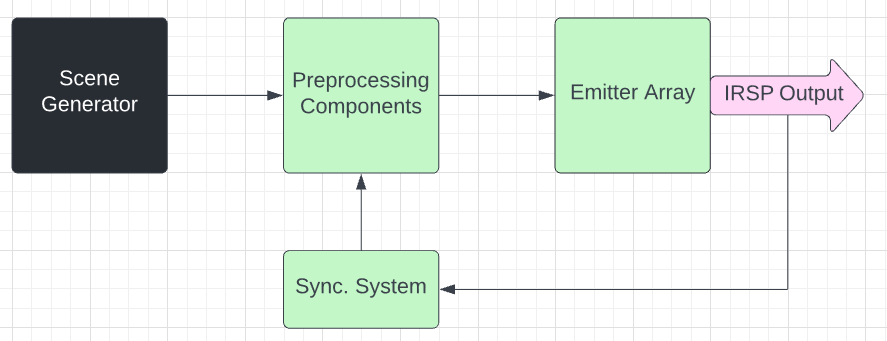
\includegraphics[width=10cm]{irsp_block_diagram}
\centering
\caption{General IRSP architecture}
\centering
\end{figure}
Testing is one of the most important aspects of any system design, as it is the bottleneck for how many reliable systems can be built \& validated. This work consists of a new approach to manually test the high-speed analog amplifier circuits within the system, as well as considerations \& redesigns for the next generation of these devices. 

\section {Motivation}
IRSPs can be characterized by multiple factors, of which two of the most important are frame rate and output temperature range. Frame rate can be described as the number of discrete outputs from the display device per second. The frame rate is directly tied to the rise time of individual pixels, which is fully dependent on the display architecture and physical properties. The temperature range represents different "colors" or ranges of IR light that the projector can display. An ideal device has both high refresh rate and high max temperature to overcome the challenges of temperature-based projection. \cite{marks} \par
Much of the IRSP market is dominated by resistor array devices. By heating up resistors (mapped to each pixel) to specific points with controlled current input, the device can simulate temperature output for an infrared image. The use of resistors limits the benefits of this approach, however. \cite{spie:2015} Resistor arrays depend on raising temperatures to the actual desired temperature of the projected image. While innovative, resistors cannot dissipate heat quickly, limiting their rise time. The characteristics of the resistors are a hard limit on refresh rate, forcing most designs to stay under 500Hz. Additionally, higher projected temperatures will further increase the rise time, since the resistors will have to physically cool down from this temperature level. By limiting the max temperature output, designers can ensure that pixel rise time will consistently stay within a certain range. \par
Since 2008, CVORG has been at the forefront of developing an Infrared LED-based IRSP with a full suite of custom hardware and software control. \cite{peyman} The success of the current iteration of the system has allowed us to continue researching improvements and changes to the system that would further expand on the technology's potential. Our technology is now targeting a 1024 x 1024 display at 2KHz. \par
After successfully developing the technology to a certain point, it was considered stable enough to reproduce and iterate on. The process of building and testing each component of the system provides one with an intimate knowledge of the functions and requirements of individual hardware components, as well as limitations to be targeted later. \par
One of the most important links in the system's chain consists of the digital-to-analog conversion and subsequent amplification. These amplified analog signals are used to drive the display, making their functionality and speed a top priority. \cite{tianne} As such, it was imperative to create reliable testing procedures for such components. The relevant systems, components \& design methodology for this portion of the system will be described in detail below. \par
